\subsection{Latency Encoding}

\textbf{Latency Encoding:}

Implementing Latency Encoding (see \ref{ssec:latency-encoding}) on the MNIST digits dataset presents a challenge. Specifically, the distribution of pixel intensity values within each image poses a substantial difficulty.

\begin{figure}[H]
    \centering
    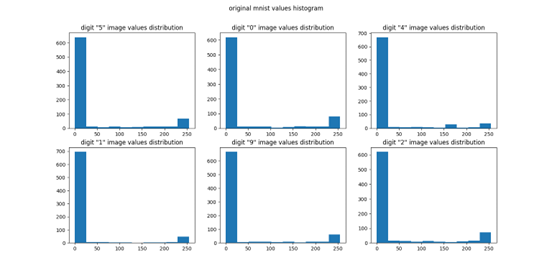
\includegraphics[width=0.8\textwidth]{methods/spike-encoding/graphs/mnist-values-histogram.png}
    \caption{histograms of the pixel values of random Mnist images divided into 10 bins}
    \label{fig:mnist-values-histogram}
\end{figure}

Although having many zero values is not a problem and can even help with achieving sparsity, we face difficulties with the distribution of non-zero values. They are often clustered around two or three key values. This becomes problematic when using linear normalization with logarithmic encoding, which is not effective in distinguishing closely situated values.

This problem is clearly depicted in the raster plot of the encoding:


\begin{figure}[H]
    \centering
    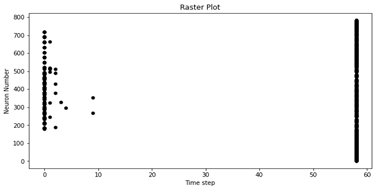
\includegraphics[width=0.8\linewidth]{methods/spike-encoding/graphs/latency-encoding-raster.png}
    \caption{raster plot of a random Mnist image encoded via latency encoding}
    \label{fig:latency-encoding-raster}
\end{figure}

To fix it, we suggest linear latency encoding by:
\begin{equation}
t(I_{\text{in}}) = -\tau \cdot \left(R \cdot I_{\text{in}} - V_{\text{thr}}\right)
\end{equation}

And clipping the zero values (they hold no useful information). The green lines represent the $\tau$ value, and the red lines represent $v_{\text{thr}}$.

\begin{figure}[H]
    \centering
    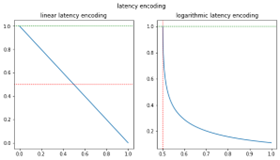
\includegraphics[width=0.5\linewidth]{methods/spike-encoding/graphs/exp-to-linear.png}
    \caption{on the right - the exponential latency encoding function, on the left - the liner latency encoding function}
    \label{fig:latency-exp-vs-lin}
\end{figure}

And as we can see, the results are significantly improved:

\begin{figure}[H]
    \centering
    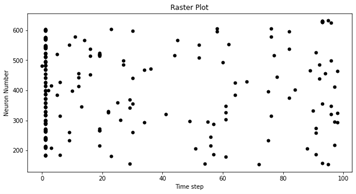
\includegraphics[width=0.7\linewidth]{methods/spike-encoding/graphs/latency-encoding-raster-linear.png}
    \caption{ raster plot of a random Mnist image encoded via linear latency encoding}
    \label{fig:latency-encoding-raster-linear}
\end{figure}